
%(BEGIN_QUESTION)
% Copyright 2010, Tony R. Kuphaldt, released under the Creative Commons Attribution License (v 1.0)
% This means you may do almost anything with this work of mine, so long as you give me proper credit

Suppose we have an Allen-Bradley model ``SLC 500'' PLC connected to a three process switches and a motor contactor as shown in this illustration:

$$\includegraphics[width=15.5cm]{i04542x01.eps}$$

Suppose the process temperature is 190 $^{o}$F, the liquid level is 3.2 feet, and the pressure is 40 PSI.  An offline view (no status color highlighting shown) of the PLC's program is as follows:

$$
\includegraphics[width=15.5cm]{i04542x02.eps}$$

Instead of the motor starting, it remains de-energized.  Determine at least three electrical faults that could prevent the motor from starting.

\vskip 20pt \vbox{\hrule \hbox{\strut \vrule{} {\bf Suggestions for Socratic discussion} \vrule} \hrule}

\begin{itemize}
\item{} What diagnostic indications might a technician look for to identify the nature of the problem?
\end{itemize}

\underbar{file i04542}
%(END_QUESTION)





%(BEGIN_ANSWER)

\noindent
{\bf Possible faults:} (not an exhaustive list)

\begin{itemize}
\item{} Tripped overload (OL) block
\item{} Open fault in output circuit
\item{} Loss of 3-phase power to motor 
\item{} Open fault in level switch input circuit
\item{} Open fault in pressure switch input circuit
\item{} Shorted temperature switch contacts
\item{} Shorted temperature switch contacts
\end{itemize}

%(END_ANSWER)





%(BEGIN_NOTES)

The process conditions are such that the PLC's output {\tt O:1/7} {\it should} be energized.  Therefore, any fault in the input switches or wiring preventing the three requisite input bit states from occurring, or any fault in the contactor or output wiring preventing the activated output from energizing the contactor, is plausible.


\vskip 20pt \vbox{\hrule \hbox{\strut \vrule{} {\bf Virtual Troubleshooting} \vrule} \hrule}

This question is a good candidate for a ``Virtual Troubleshooting'' exercise.  Presenting the diagram to students, you first imagine in your own mind a particular fault in the system.  Then, you present one or more symptoms of that fault (something noticeable by an operator or other user of the system).  Students then propose various diagnostic tests to perform on this system to identify the nature and location of the fault, as though they were technicians trying to troubleshoot the problem.  Your job is to tell them what the result(s) would be for each of the proposed diagnostic tests, documenting those results where all the students can see.

During and after the exercise, it is good to ask students follow-up questions such as:

\begin{itemize}
\item{} What does the result of the last diagnostic test tell you about the fault?
\item{} Suppose the results of the last diagnostic test were different.  What then would that result tell you about the fault?
\item{} Is the last diagnostic test the best one we could do?
\item{} What would be the ideal order of tests, to diagnose the problem in as few steps as possible?
\end{itemize}

\vfil \eject

\noindent
{\bf Prep Quiz:}

$$\includegraphics[width=15.5cm]{i04542x01.eps}$$

Examine the program for this Allen-Bradley PLC as it appears printed on paper, and determine the necessary process conditions to start the motor:

$$
\includegraphics[width=15.5cm]{i04542x03.eps}$$

\begin{itemize}
\item{} Temperature {\bf below} 179 $^{o}$F or {\bf above} 179 $^{o}$F?
\vskip 10pt
\item{} Level {\bf below} 4 feet or {\bf above} 4 feet?
\vskip 10pt
\item{} Pressure {\bf below} 33 PSI or {\bf above} 33 PSI?
\end{itemize}

\vskip 10pt

(Make one choice for {\it each} process switch)


\vfil \eject

\noindent
{\bf Prep Quiz:}

$$\includegraphics[width=15.5cm]{i04542x01.eps}$$

Examine the program for this Allen-Bradley PLC as it appears printed on paper, and determine the necessary process conditions to start the motor:

$$
\includegraphics[width=15.5cm]{i04542x04.eps}$$

\begin{itemize}
\item{} Temperature {\bf below} 179 $^{o}$F or {\bf above} 179 $^{o}$F?
\vskip 10pt
\item{} Level {\bf below} 4 feet or {\bf above} 4 feet?
\vskip 10pt
\item{} Pressure {\bf below} 33 PSI or {\bf above} 33 PSI?
\end{itemize}

\vskip 10pt

(Make one choice for {\it each} process switch)


%INDEX% PLC, relating I/O status to virtual elements

%(END_NOTES)


